% Exam Template for UMTYMP and Math Department courses
%
% Using Philip Hirschhorn's exam.cls: http://www-math.mit.edu/~psh/#ExamCls
%
% run pdflatex on a finished exam at least three times to do the grading table on front page.
%
%%%%%%%%%%%%%%%%%%%%%%%%%%%%%%%%%%%%%%%%%%%%%%%%%%%%%%%%%%%%%%%%%%%%%%%%%%%%%%%%%%%%%%%%%%%%%%

% These lines can probably stay unchanged, although you can remove the last
% two packages if you're not making pictures with tikz.
\documentclass[11pt]{exam}
\RequirePackage{amssymb, amsfonts, amsmath, latexsym, verbatim, xspace, setspace, blkarray, multirow, array}
\RequirePackage{tikz, pgflibraryplotmarks, pgfplotstable}
\RequirePackage{booktabs,pgfplots,pgfplotstable}

% By default LaTeX uses large margins.  This doesn't work well on exams; problems
% end up in the "middle" of the page, reducing the amount of space for students
% to work on them.
\usepackage[margin=1in]{geometry}


% Here's where you edit the Class, Exam, Date, etc.
\newcommand{\class}{Simulaci\'on}
\newcommand{\code}{}
\newcommand{\term}{Primavera 2019}
\newcommand{\examnum}{Tarea 2}
%\newcommand{\examdate}{01/10/18}
\newcommand{\timelimit}{02/10/18}

% For an exam, single spacing is most appropriate
\singlespacing
% \onehalfspacing
% \doublespacing

% For an exam, we generally want to turn off paragraph indentation
\parindent 0ex

%
\begin{document} 

% These commands set up the running header on the top of the exam pages
\pagestyle{head}
\firstpageheader{}{}{}
\runningheader{\class}{\examnum\ - P\'agina \thepage\ de \numpages}{\examdate}
\runningheadrule

\begin{flushright}
\begin{tabular}{p{2.8in} r l}
\textbf{\class} & \textbf{Nombre:} & \makebox[2in]{\hrulefill}\\
\textbf{\code} && \textbf{C\'odigo de honor:} \\
\textbf{\term} && No hemos dado ni recibido\\
\textbf{\examnum} && ayuda durante esta Tarea\\
\textbf{\examdate} && \\
\textbf{Fecha de Entrega: \timelimit} & \textbf{Firma} & \makebox[2in]{\hrulefill}
\end{tabular}\\
\end{flushright}
\rule[1ex]{\textwidth}{.1pt}


Este certamen contiene \numpages\ p\'aginas (incluyendo esta cubierta) y 
\numquestions\ preguntas.  Cerciorece que su copia contiene todas las p\'aginas.  Ponga su iniciales arriba de cada p\'agina en el caso de que separe las hojas y estas se puedan perder.\\

Usted \textbf{PUEDE} utilizar una hoja A4 escrita en una de sus carillas para el certamen.\\

Se requiere que muestre su trabajo para cada problema en este certamen.  Las siguientes reglas aplican:\\

\begin{minipage}[t]{3.7in}
\vspace{0pt}
\begin{itemize}

\item \textbf{Organize su trabajo}, de forma razonablemente ordenada, en el espacio entregado. Trabajo desorganizado dif\'icil de evaluar recibir\'a poco o nada de puntaje (independiente de su exactitud). 

\item \textbf{Respuestas misteriosas o sin fundamentos no recibir\'an puntaje}.  Una respuesta correcta, sin soporte de calculos, explicaci\'on, o trabajo algebraico \textbf{NO} recibir\'a puntaje; una respuesta incorrecta que sea el resultado de calculos intermedios correctos podr\'ia recibir puntaje parcial.

\item Si necesita mas espacio, use el reverso de la p\'agina; indique claramente cuando haga esto.
\end{itemize}

No escriba en la tabla a la derecha.
\end{minipage}
\hfill
\begin{minipage}[t]{2.3in}
\vspace{0pt}
%\cellwidth{3em}
\gradetablestretch{2}
\vqword{Problem}
\addpoints % required here by exam.cls, even though questions haven't started yet.	
\gradetable[v]%[pages]  % Use [pages] to have grading table by page instead of question

\end{minipage}
\newpage % End of cover page

%%%%%%%%%%%%%%%%%%%%%%%%%%%%%%%%%%%%%%%%%%%%%%%%%%%%%%%%%%%%%%%%%%%%%%%%%%%%%%%%%%%%%
%
% See http://www-math.mit.edu/~psh/#ExamCls for full documentation, but the questions
% below give an idea of how to write questions [with parts] and have the points
% tracked automatically on the cover page.
%
%
%%%%%%%%%%%%%%%%%%%%%%%%%%%%%%%%%%%%%%%%%%%%%%%%%%%%%%%%%%%%%%%%%%%%%%%%%%%%%%%%%%%%%
\begin{questions}
\section*{Probability theory}
% Basic question
\addpoints
\question Una variable aleatoria $Y$ tiene la siguiente funci\'on de densidad:

 \[f_Y(x)=
\begin{cases}
0&\text{for $x < 0$}\\
\frac{3}{16}x^2+\frac{1}{4}& \text{for $0\leq x < 2$}\\
0&\text{for $2 < x$}\\
\end{cases}
\]

\begin{parts}
\part[4] ?`Cu\'al es el valor esperado de Y?
%\fillwithlines{1.5 in}
\fillwithlines{3.5 in}
\part[6] ?`Cu\'al es la funci\'on de densidad acumulada de Y? ?`Es m\'as probable obtener un valor cercano a $1/2$ o a $3/2$?%\fillwithlines{3 in}
\fillwithlines{3 in}
\end{parts}
% Basic question

\newpage
\addpoints
\question Una m\'aquina produce componentes que son ya sea aceptables o defectuosos. Despu\'es de observar 100 pares de componentes, la siguiente informaci\'on fue recolectada:


 \begin{table}[h!]
	\centering
    \setlength{\extrarowheight}{2pt}
    \begin{tabular}{cc|c|c|}
      & \multicolumn{1}{c}{} & \multicolumn{2}{c}{Segundo}\\
      & \multicolumn{1}{c}{} & \multicolumn{1}{c}{Aceptable}  & \multicolumn{1}{c}{Defectuoso} \\\cline{3-4}
      \multirow{2}*{Primero}  & Aceptable & 75 & 5 \\\cline{3-4}
      & Defectuoso & 10 & 10 \\\cline{3-4}
    \end{tabular}
  \end{table}


Dej\'emos que $X_1$ represente el primer componente y $X_2$ el segundo. Los trabajadores asignaron el valor 0 a un componente aceptable y el de 1 a un componente defectuoso. Conteste las siguientes preguntas:
\begin{parts}
\part[4] Estime la funci\'on de probabilidad de masa conjunta para estas dos variables aleatorias.
%\fillwithlines{1.5 in}
\fillwithlines{2.5 in}
\part[6] ?`Cu\'al es la probabilidad que el segundo componente sea defectuoso si el primer componente no es defectuoso? ?`Cu\'al es la probabilidad que el segundo componente sea defectuoso? ?`Son $X_1$ y $X_2$ independientes?%\fillwithlines{3 in}
\fillwithlines{2.5 in}
\end{parts}


\section*{C\'alculo de m\'etricas en simulaci\'on}
\question Usted decide testear si su entendimiento sobre como opera internamente una simulaci\'on es el adecuado. Para ello va a un restaurant y comienza a observar su operaci\'on y va registrando lo que ve en una hoja, tal como se observa en la Figura \ref{fig:esttiemp}.
\begin{figure}[htbp]
\centering
	%trim={<left> <lower> <right> <upper>}
	%[width=6.5cm, height=5.5cm]
		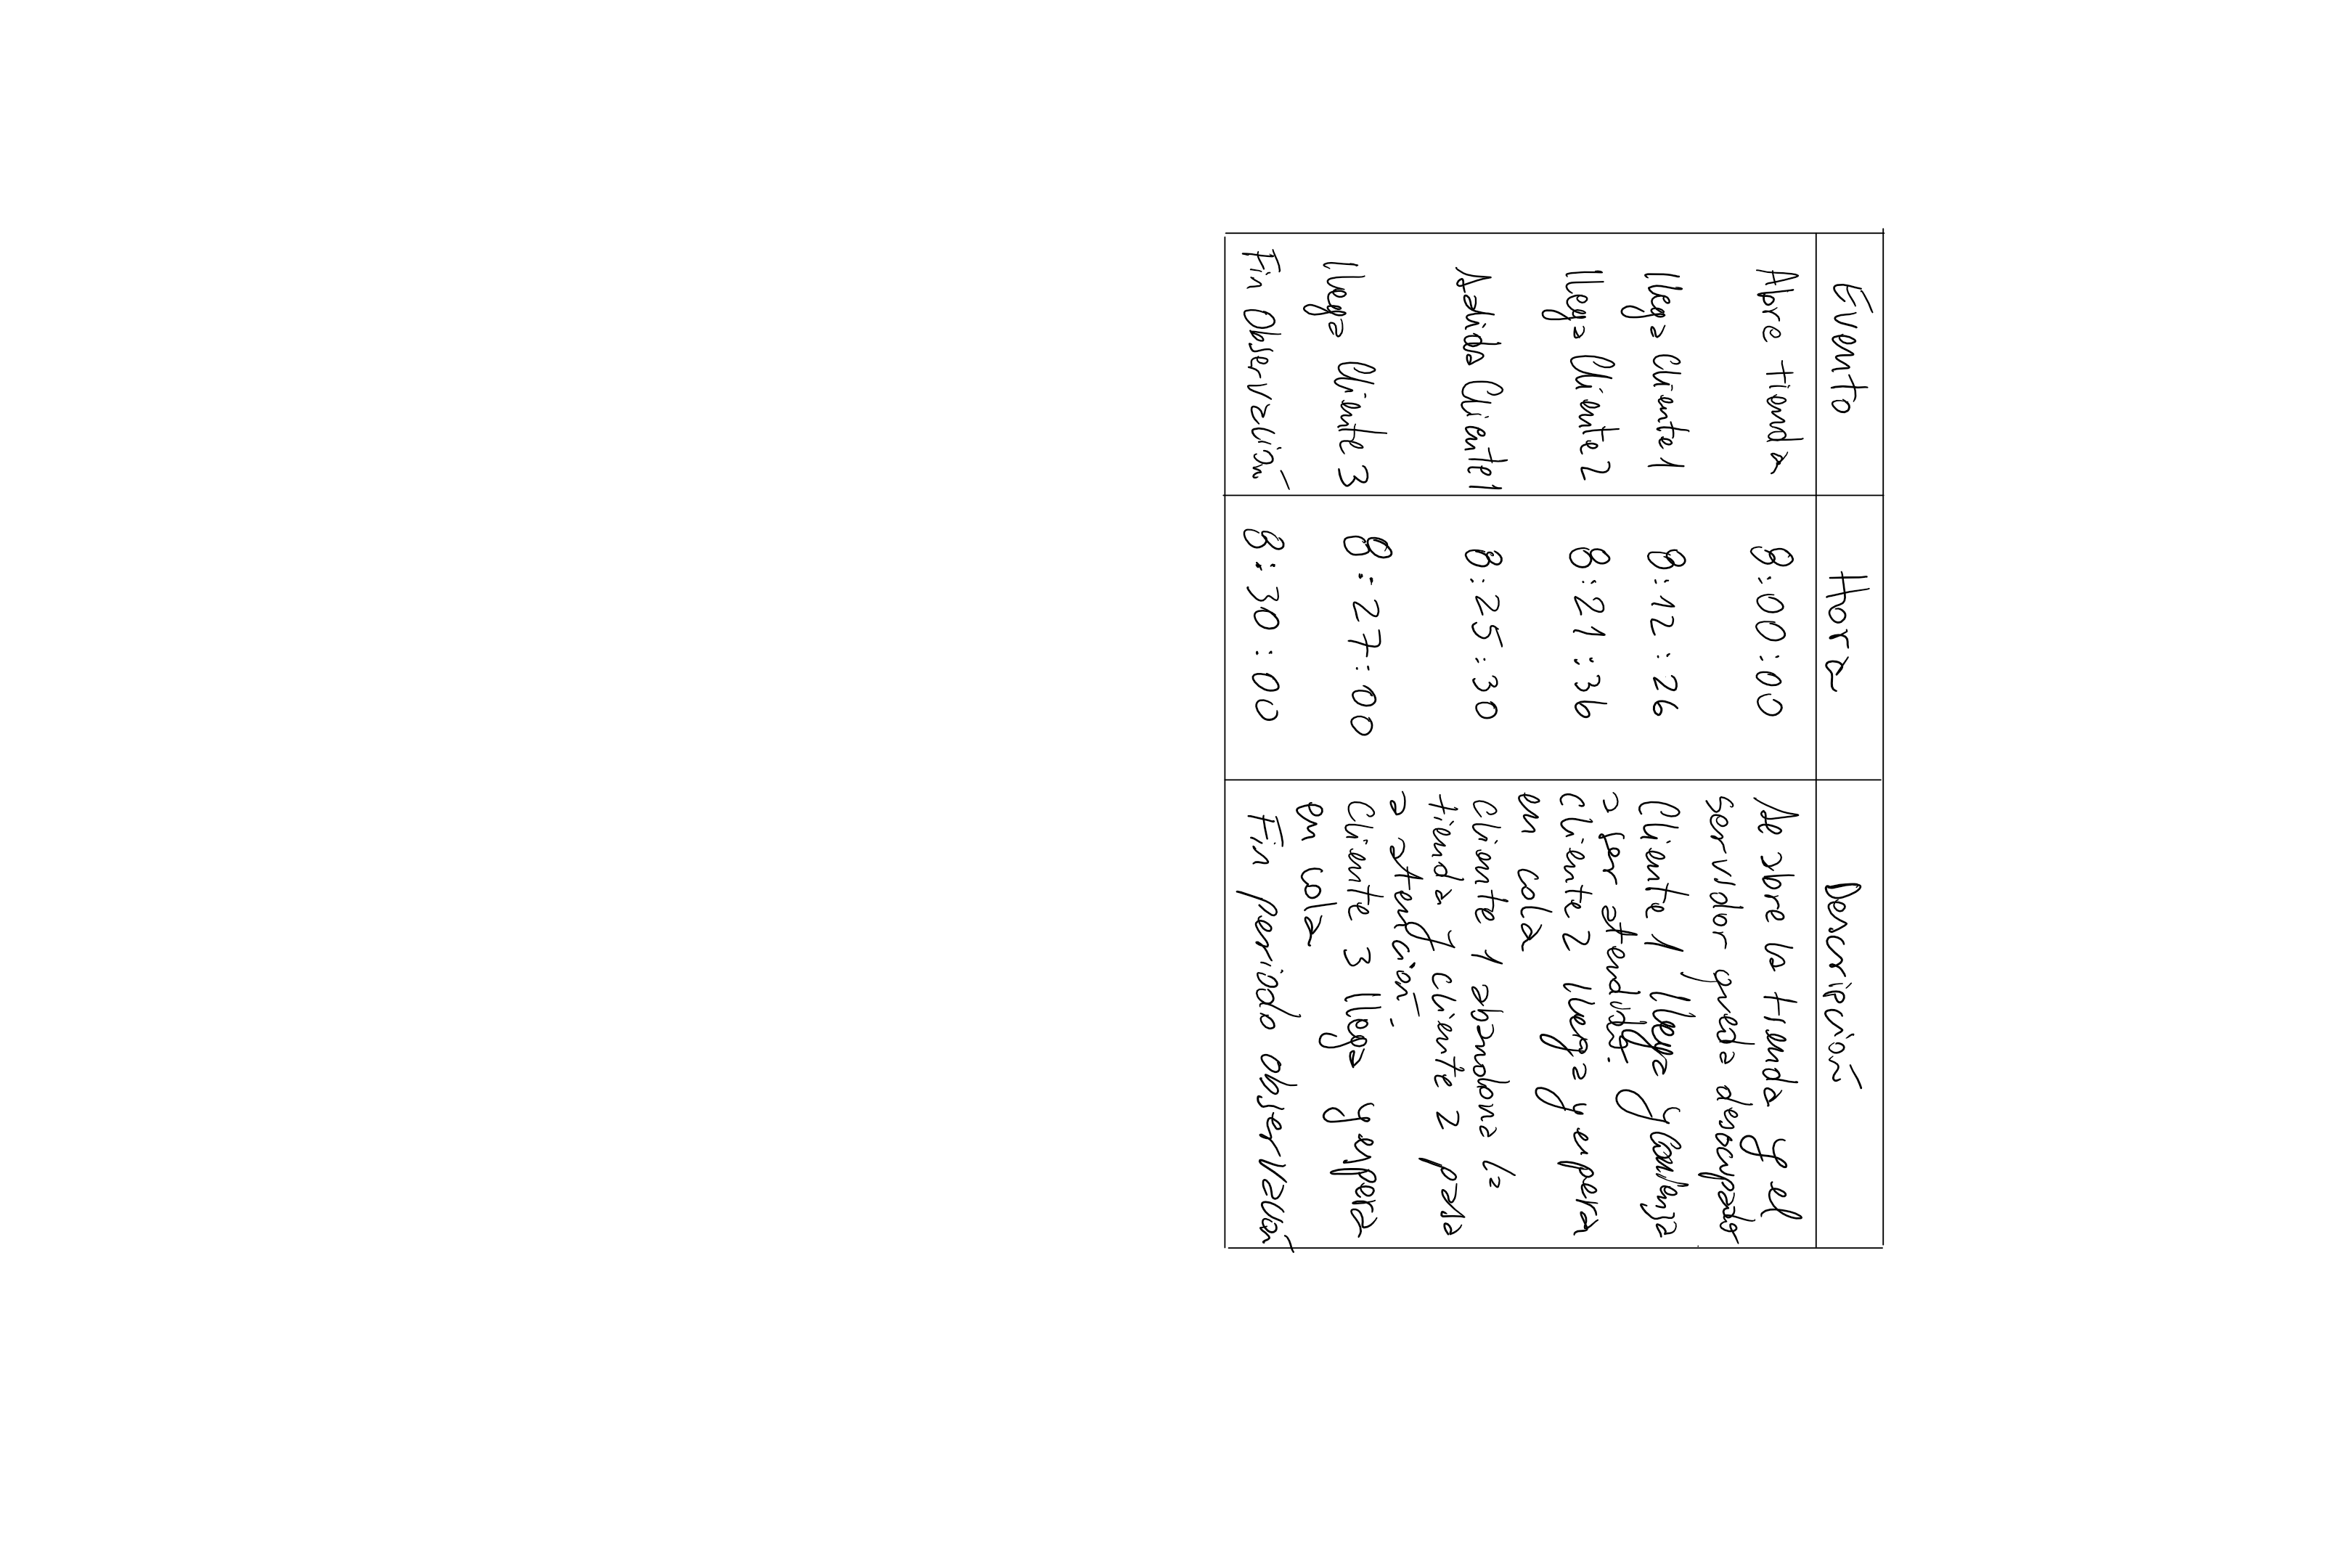
\includegraphics[scale=0.7,keepaspectratio,trim={22cm 4cm 8.5cm 4cm},clip,angle =90]{dic1.png}
			\caption{Formulario de asignaci\'on de estudio de tiempos}
			\label{fig:esttiemp}
\end{figure}

\begin{parts}
\part[3] ?`Cu\'al es el tiempo promedio en el sistema?
\fillwithlines{3 in}
\part[8] ?`Cu\'al es n\'umero promedio en el sistema?
\fillwithlines{4 in}
\part[4] ?`Cu\'al es la utilizaci\'on del servidor?
\fillwithlines{3 in}
\end{parts}

\newpage
\section*{Validaci\'on de distribuci\'on}

\question Usted recolect\'o 1000 observaciones de demanda de un determinado producto. Tal como aprendi\'o en simulaci\'on hizo un histograma para observar como se agrupaba la informaci\'on. Adem\'as usted sabe que debe ajustar una distribuci\'on te\'orica con tal de remplazar la informaci\'on del histograma. Despu\'es de unos cuantos an\'alisis usted ha llegado a la informaci\'on de la Figura \ref{fig:chi2}.
 
\begin{figure}[htbp]
\centering
	%trim={<left> <lower> <right> <upper>}
	%[width=6.5cm, height=5.5cm]
		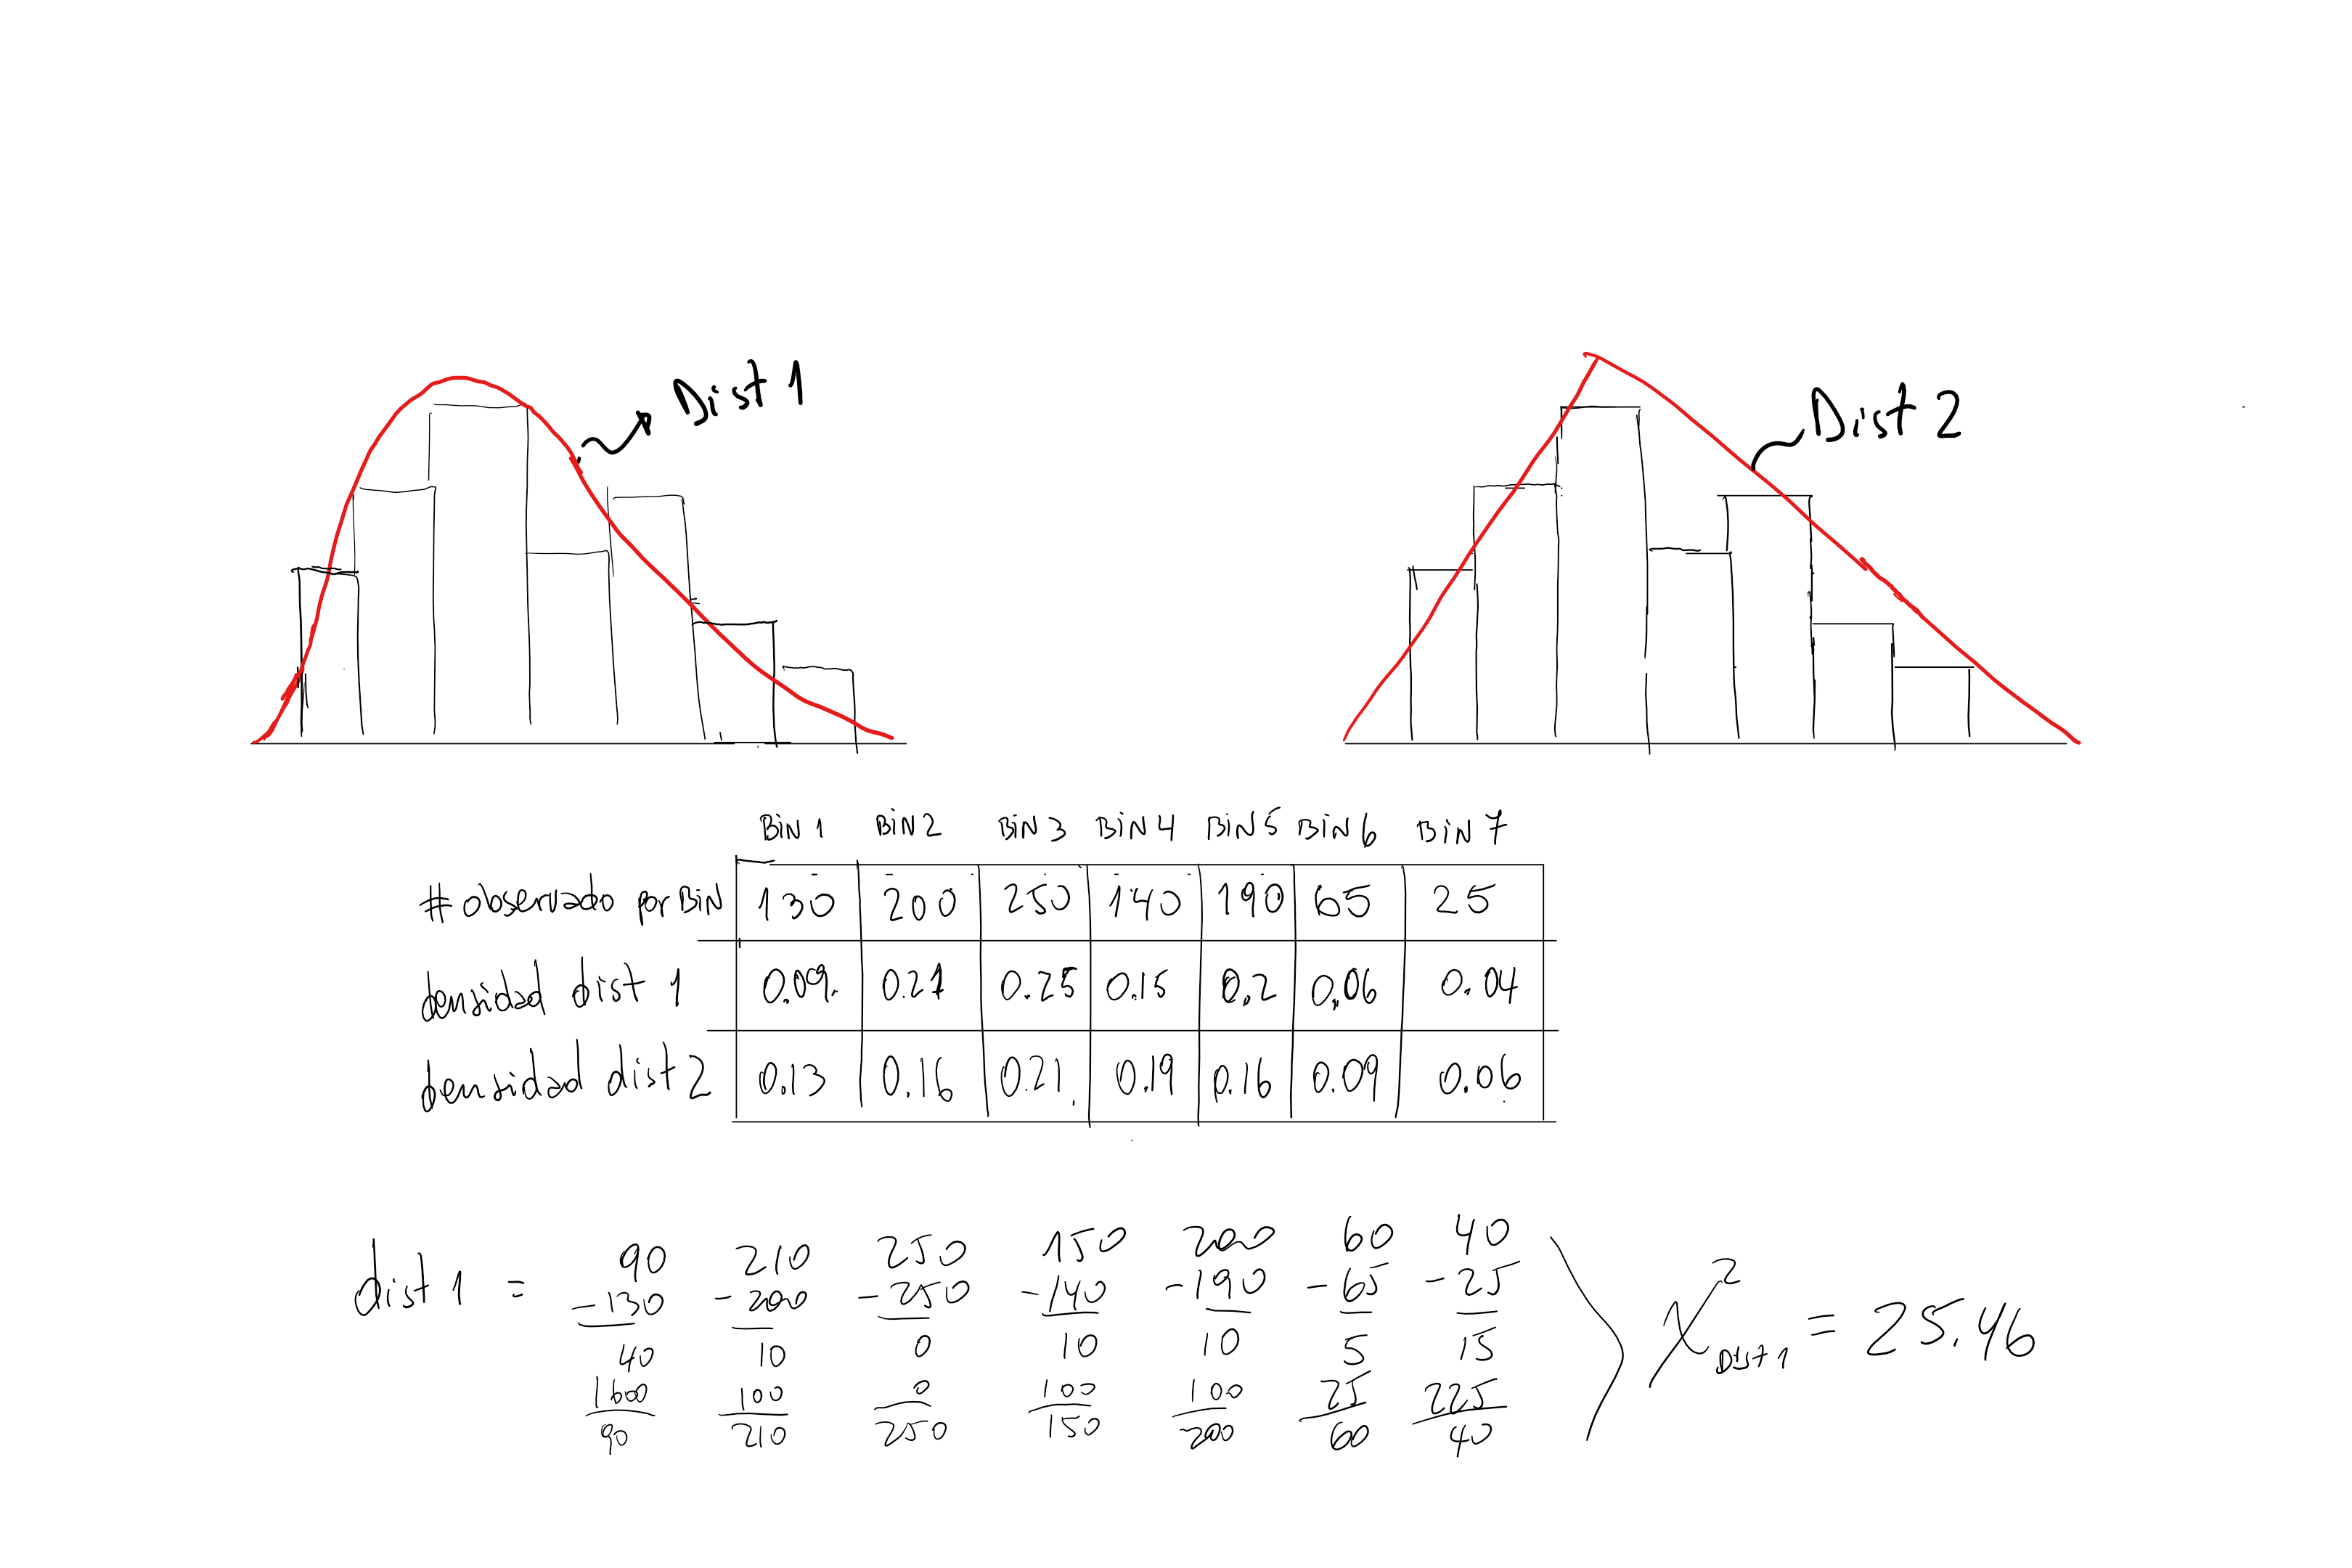
\includegraphics[scale=0.43,keepaspectratio,trim={2cm 7cm 6cm 2cm},clip,angle =0]{chi2.png}
			\caption{Formulario de asignaci\'on de estudio de tiempos}
			\label{fig:chi2}
\end{figure}

\begin{parts}
\part[9] Calcular el valor $\tilde{\chi}^2$ para cada una de las distribuciones.
\fillwithlines{5 in}
\part[4] Si el valor $\chi^2$ de tabla es 19.67, ?`son adecuadas las distribuciones?
\fillwithlines{2 in}
\part[3] Un amigo le comenta que aumentando el nivel de significancia ($\alpha$) usted podr\'ia tomar otra decisi\'on. ?`Est\'a su amigo en lo correcto?
\fillwithlines{1 in}
\end{parts}

\question Usted quiere modelar el n\'umero diario de clientes que van a un restaurant. El due\~no del local entrega una aproximaci\'on te\'orica de como los clientes se distribuyen durante la semana:

\begin{table}[!htbp]
\centering
\begin{tabular}{lcccccc}
\toprule
D\'ia&L&M&M&J&V&S\\
\midrule
Porcentaje (\%) & 15 & 10 & 15 & 20 & 25 & 15\\
\bottomrule
\end{tabular}
\end{table}

Antes de utilizar esta distribuci\'on te\'orica usted decide validarla, por lo cual va a recolectar datos y obtiene la siguiente tabla:

\begin{table}[!htbp]
\centering
\begin{tabular}{lccccccc}
\toprule
D\'ia&L&M&M&J&V&S&Total\\
\midrule
N\'umero de Clientes & 26 & 18 & 34 & 45 & 50 & 27 & 200\\
\bottomrule
\end{tabular}
\end{table}

\begin{parts}
\part[16] Comprobar si la distribuci\'on te\'orica sirve para modelar el flujo de clientes
\fillwithlines{3 in}
\end{parts}
\newpage
\section*{Likelihood y moment matching}
%\iffalse
\question Suponga que $X$ es una variable aleatoria discreta con funci\'on de probabilidad de masa.

\begin{table}[!htbp]
\centering
\begin{tabular}{lcccc}
\toprule
X&0&1&2&3\\
\midrule
$P(X=x)$ & $2\theta/3$ & $\theta/3$& $2(1-\theta)/3$ & $(1-\theta)/3$\\
\bottomrule
\end{tabular}
\end{table}

\begin{parts}
\part[16] Se han obtenido diez muestras de la distribuci\'on (3,0,2,1,3,2,1,0,2,1), y se le pide determinar el par\'ametro $\hat{\theta}$.
\fillwithlines{6 in}
\newpage
\end{parts}

%\iffalse
\question Se le pide determinar el estimador de ``maximum likelihood'' que caracteriza el par\'ametro \'optimo de una distribuci\'on exponencial. La funci\'on de densidad se presenta a continuaci\'on.

\[f(x)=
\begin{cases}
\lambda_0 ~\text{exp}(-\lambda_0x_j)&\text{for $x\in[0,\infty)$}\\
0&\text{de otro modo}\\
\end{cases}
\]

\begin{parts}
\part[12] Determine el par\'ametro $\hat{\lambda_0}$.
\fillwithlines{4 in}
\part[3] ?`Que diferencia hay entre el par\'ametro calculado en (a) y el valor obtenido por medio del m\'etodo de ``Moment Matching''
\fillwithlines{1 in}
\end{parts}
%\fi
\section*{Ajuste de distribuciones cuando no hay datos}
\question En esta secci\'on se eval\'ua su entendimiento del que hacer cuando no se dispone de datos.
\begin{parts}
\part[3] En una distribuci\'on Beta, si se cumple que  $\alpha_1 > \alpha_2$ y ambos son mayores que 1, ?`qu\'e forma toma la distribuci\'on?
\fillwithlines{2 in}
\part[3] En una distribuci\'on Beta, si los par\'ametros $\alpha_1$ y $\alpha_2$ son ambos menores a 1, ?`qu\'e forma toma la distribuci\'on?
\fillwithlines{2 in}
\part[6] Usted quiere modelar un proceso y no se mantienen registros de cuanto \'este demora. Un operario le dice que como m\'inimo el proceso demora 5 minutos, que el valor mas observado por \'el es de 9 minutos, y que el valor m\'as at\'ipico que ha visto es 15 minutos. Ajuste una distribuci\'on Beta para este proceso.
\fillwithlines{3 in}
\end{parts}
\end{questions}
\end{document}